\begin{frame}
  \frametitle{Let do engineering \ldots}
  \begin{center}
    As computers cannot boot without an Office Pack \\[1em]
    \begin{tikzpicture}
      \node[inner sep=0pt] at (0,0) {\includegraphics[width=25mm]{images/mouse.jpg}};
      \node[inner sep=0pt] at ( 30:25mm) {\includegraphics[width=25mm]{images/excel.png}};
      \node[inner sep=0pt] at (150:25mm) {\includegraphics[width=25mm]{images/word.png}};
      % \node[inner sep=0pt] at (270:17.5mm) {\includegraphics[width=25mm]{images/airbus-land-off.jpg}};
    \end{tikzpicture} \\[.5em]
    Students and later engineers know \\[.5em]
    You can do \textbf{everything} with it at work \\[.5em]
    from R\&D to communication, database, accounting, \ldots \\[1em]
    You will Excel !!!
  \end{center}
\end{frame}

\begin{frame}[fragile]
  \frametitle{Mouse Algorithm}
  \begin{columns}[T]
    \begin{column}{.4\textwidth}
      \includegraphics[width=1.\textwidth]{images/excel-sheet.png}
    \end{column}
    \begin{column}{.6\textwidth}
      \small
      How to compute the derivative of a set of measures ?
      \begin{enumerate}
      \item copy the data of the first column
      \item past to the second column starting from the second line
      \item enter the formulae $(A-B)/dt$ in the third column
      \end{enumerate}
      \textbf{Easy and Efficient ! Isn't it ? } \\[1em]
      Next exercise compute an histogram \ldots \\[1em]
      {\tiny Python answer if you are lazy
        % \reflectbox{
        % \scalebox{1}[-1]{
\begin{Verbatim}
for value in values:
    hist[value // bin_size] += 1
\end{Verbatim}
        }%}
    \end{column}
  \end{columns}
  \vspace{3em}
  \centerline{\alert{But in fact here : License Cost $\ll$ Salary}}
\end{frame}

\begin{frame}
  \frametitle{A cabinetworker as a lot of tools !}
  \begin{center}
    \includegraphics[height=5cm]{images/ebeniste.jpg} \\[1em]
    \textbf{Why teach and do stupid things?}
  \end{center}
\end{frame}

\begin{frame}
  \frametitle{Open Source Community has a lot of tools !}
  \begin{columns}[T]
    \begin{column}{.5\textwidth}
      Of course if you have to build this \\[1em]
      \begin{center}
        \includegraphics[width=.8\textwidth]{images/airbus-land-off.jpg} \\[1em]
      \end{center}
      You need the right tools \\
      Doesn't matter how it cost \\
      And Open Source is or not so important
    \end{column}
    \begin{column}{.5\textwidth}
      But for teaching, learning or DIY \\[1em]
      You can find what you are looking for \\
      And maybe discover alternatives \\[1em]
      \textbf{Like to simulate electronic circuit \\
        or even complex systems} \\[1em]
      You can get it \\
      even if you live in a ghetto \\
      It's free and open !
    \end{column}
  \end{columns}
\end{frame}

\begin{frame}
  \frametitle{Simulation Workflow}
  % \begin{center}
  %   \begin{tabular}{ccccc}
  %     Steer & $\longrightarrow$ & Process & $\longrightarrow$ & Analyse \\[2em]
  %     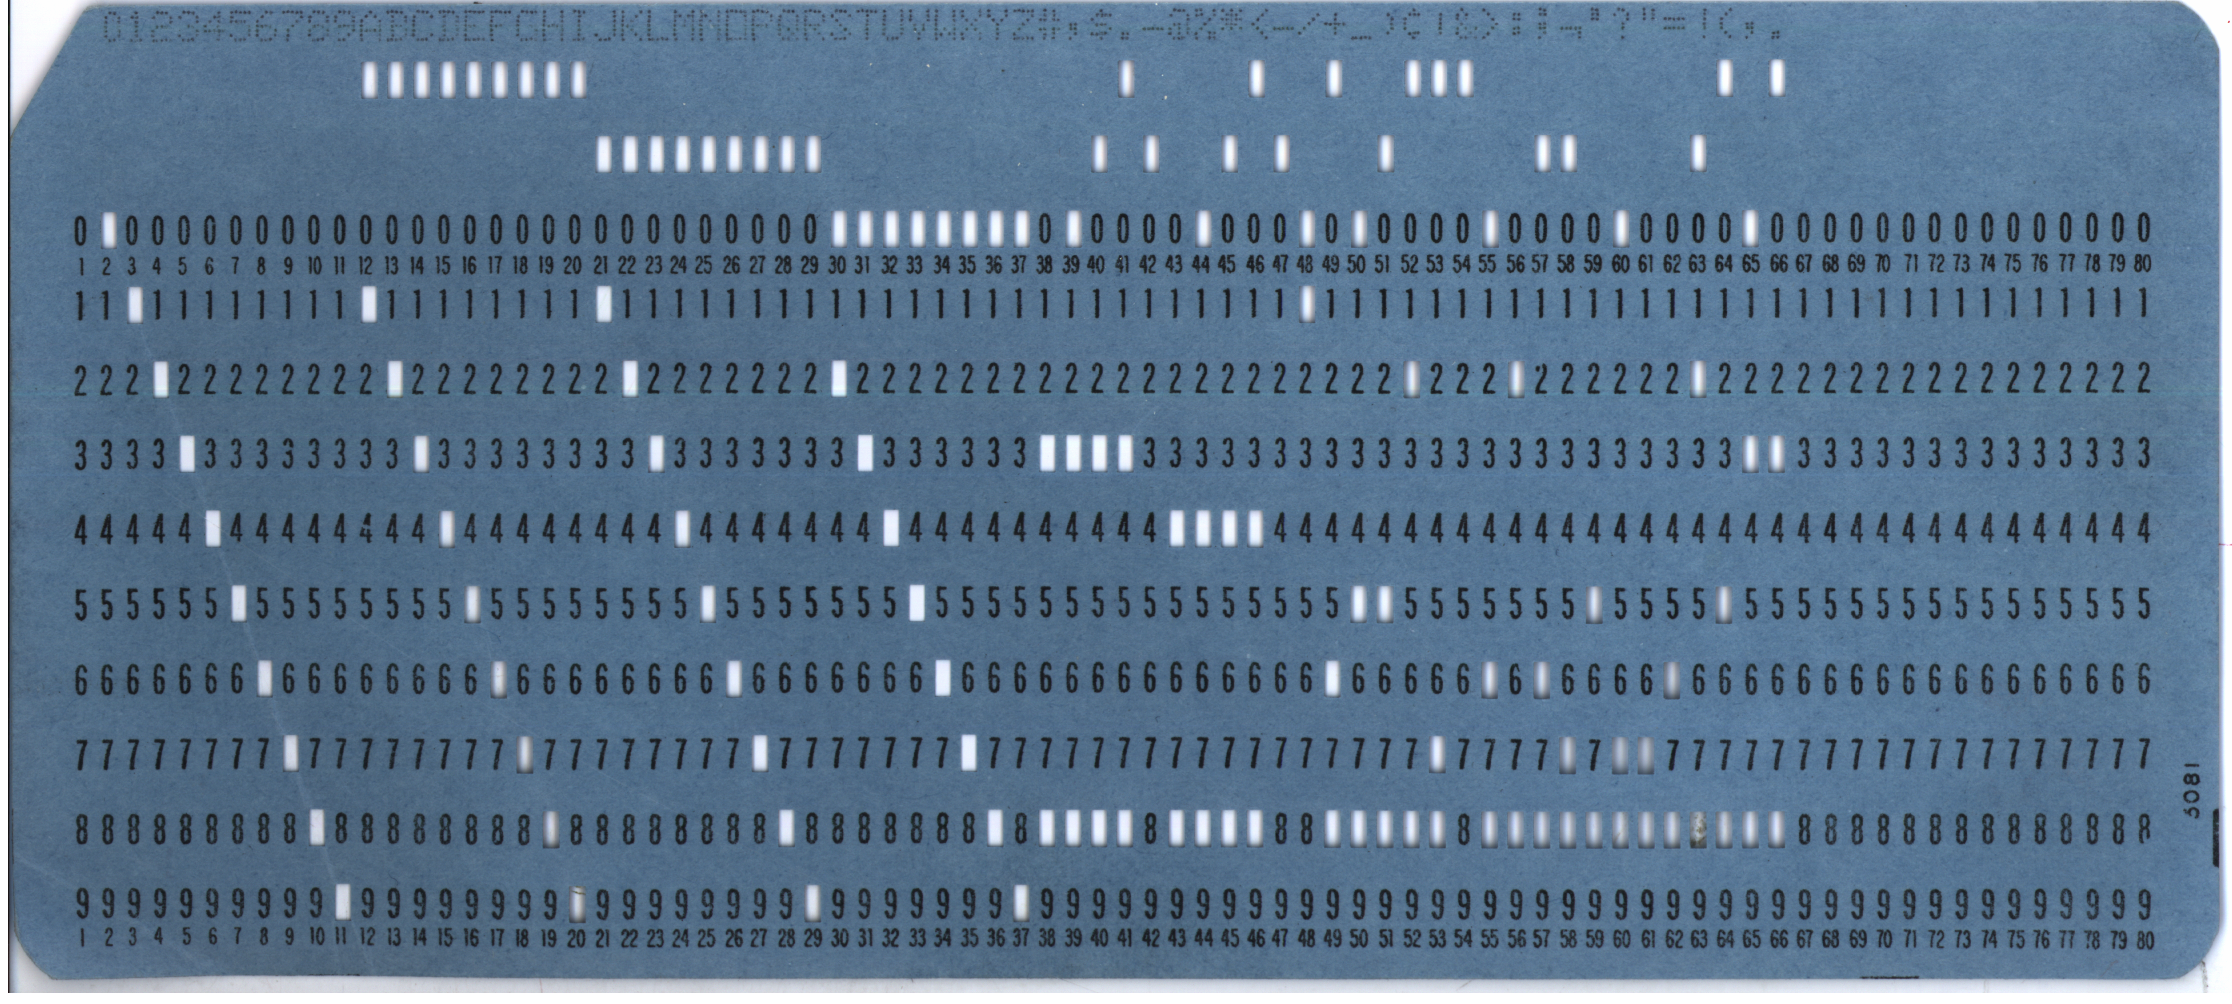
\includegraphics[width=.25\textwidth]{images/punch-card.png} & &
  %     \includegraphics[width=.25\textwidth]{images/eniac.jpg} & &
  %     \includegraphics[width=.25\textwidth]{images/mainframe-console.jpg}
  %   \end{tabular}
  % \end{center}
  \begin{columns}
    \begin{column}{.3\textwidth}
      \centerline{Steer}
    \end{column}
    \begin{column}{.05\textwidth}
    \end{column}
    \begin{column}{.3\textwidth}
      \centerline{Process}
    \end{column}
    \begin{column}{.05\textwidth}
    \end{column}
    \begin{column}{.3\textwidth}
      \centerline{Analyse}
    \end{column}
  \end{columns}
  \begin{columns}
    \begin{column}{.3\textwidth}
      \begin{center}
        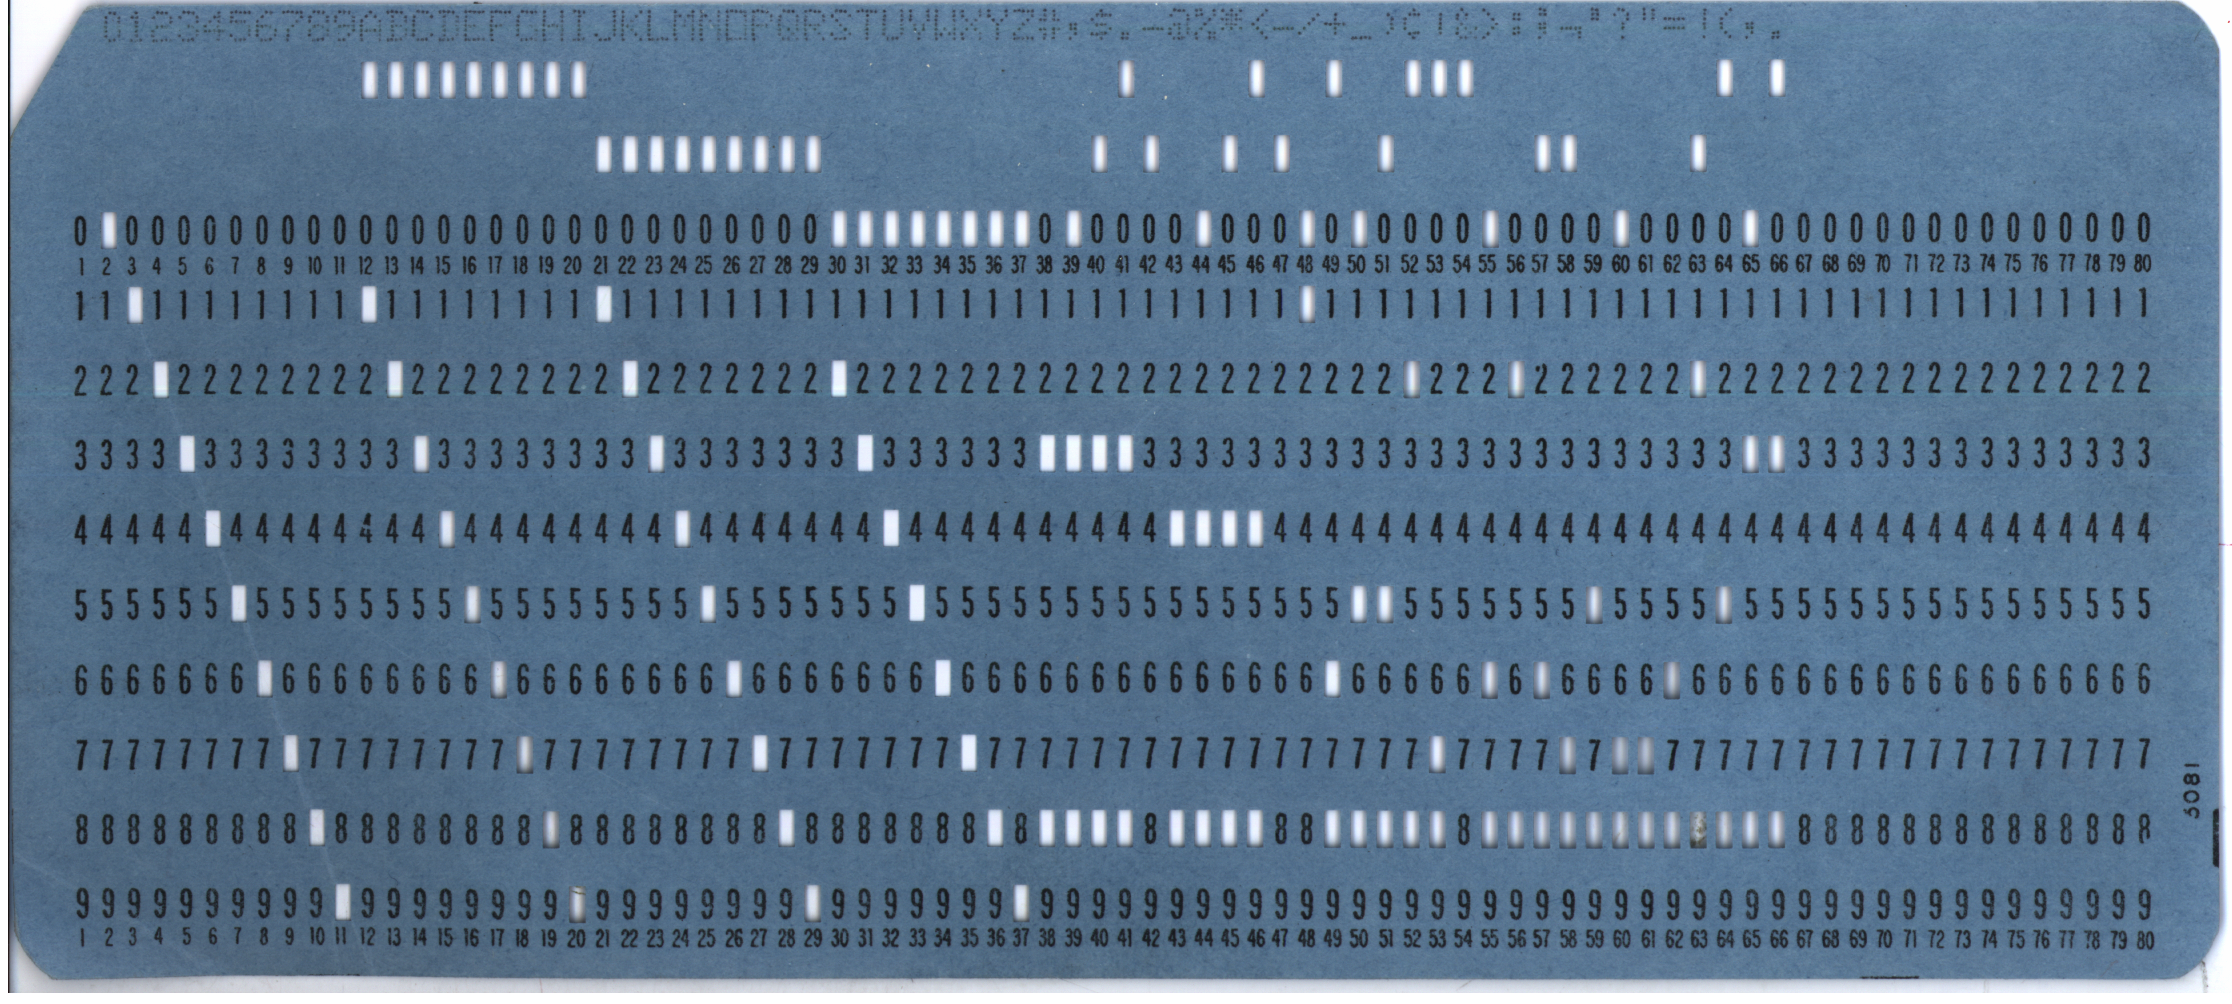
\includegraphics[width=.9\textwidth]{images/punch-card.png}
      \end{center}
    \end{column}
    \begin{column}{.05\textwidth}
      \centerline{$\longrightarrow$}
    \end{column}
    \begin{column}{.3\textwidth}
      \begin{center}
        \includegraphics[width=.9\textwidth]{images/eniac.jpg}
      \end{center}
    \end{column}
    \begin{column}{.05\textwidth}
      \centerline{$\longrightarrow$}
    \end{column}
    \begin{column}{.3\textwidth}
      \begin{center}
        \includegraphics[width=.9\textwidth]{images/mainframe-console.jpg}
      \end{center}
    \end{column}
  \end{columns}
\end{frame}

\begin{frame}
  \frametitle{Thanks to Guido van Rossum, We have Python !}
  \begin{columns}
    \begin{column}{.3\textwidth}
      \begin{center}
        \begin{tikzpicture}
          \begin{scope}
            \clip [rounded corners=2mm] (0,0) rectangle coordinate (centerpoint) ++(3cm,5cm);
            \node [inner sep=0pt] at (centerpoint) {\includegraphics[height=5cm]{images/guido.jpg}};
          \end{scope}
        \end{tikzpicture}
      \end{center}
    \end{column}
    \begin{column}{.7\textwidth}
      \begin{itemize}
      \item Indentation is syntax ! So clever ! \\
        {\small Look at PhD student \Cpp{} code}
      \item Canonical Syntax
      \item High Level Language
      \item Object Oriented
      \item Transparent memory management
      \item Easy to bind with C or Fortran
      \item An incredible scientific environment
      \end{itemize}
    \end{column}
  \end{columns}
\end{frame}

\begin{frame}
  \frametitle{Simulation Workflow with Python}
  \begin{columns}
    \begin{column}{.3\textwidth}
      \centerline{Steer}
    \end{column}
    \begin{column}{.05\textwidth}
    \end{column}
    \begin{column}{.3\textwidth}
      \centerline{Process}
    \end{column}
    \begin{column}{.05\textwidth}
    \end{column}
    \begin{column}{.3\textwidth}
      \centerline{Analyse}
    \end{column}
  \end{columns}
  \begin{columns}
    \begin{column}{.3\textwidth}
      \begin{center}
        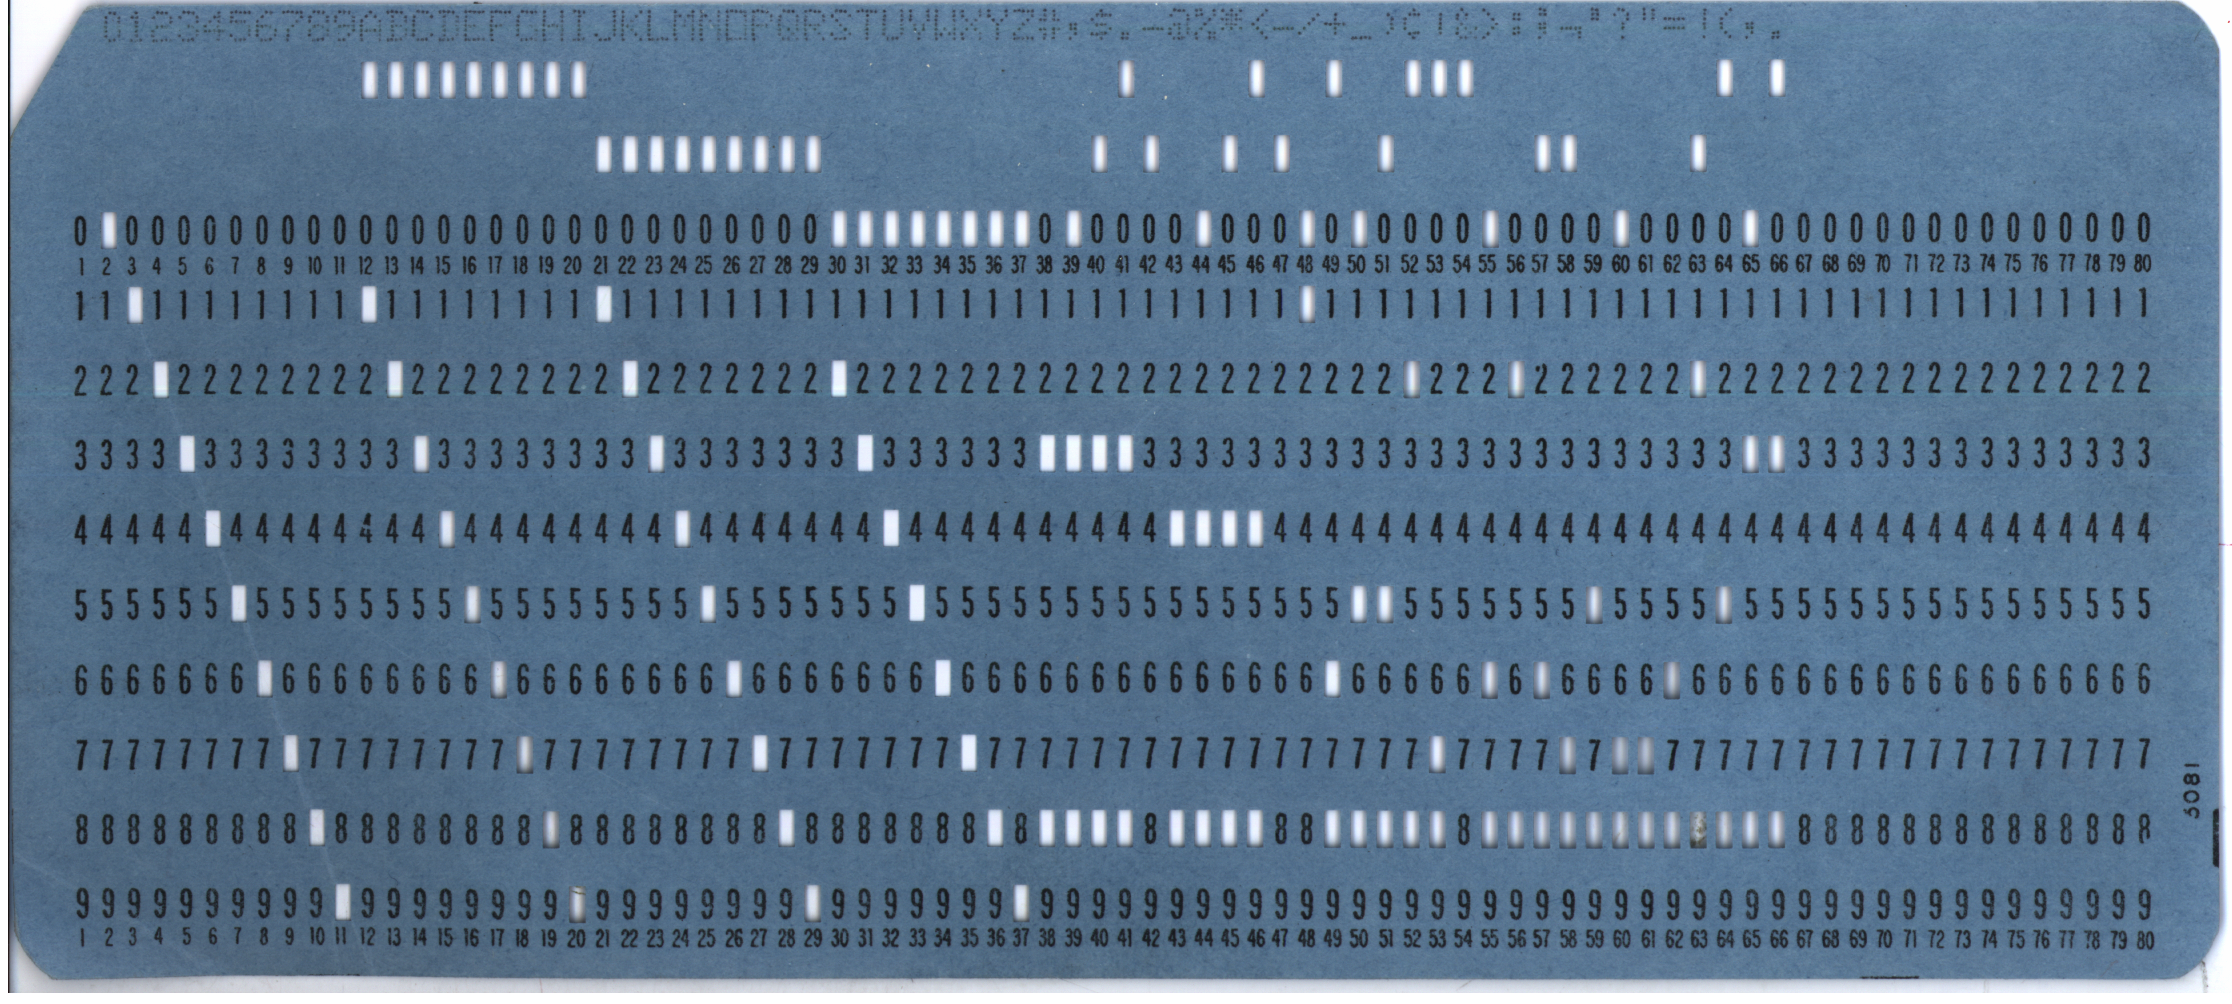
\includegraphics[width=.9\textwidth]{images/punch-card.png}
      \end{center}
    \end{column}
    \begin{column}{.05\textwidth}
      \centerline{$\longrightarrow$}
    \end{column}
    \begin{column}{.3\textwidth}
      \begin{center}
        \includegraphics[width=.9\textwidth]{images/eniac.jpg}
      \end{center}
    \end{column}
    \begin{column}{.05\textwidth}
      \centerline{$\longrightarrow$}
    \end{column}
    \begin{column}{.3\textwidth}
      \begin{center}
        \includegraphics[width=.9\textwidth]{images/mainframe-console.jpg}
      \end{center}
    \end{column}
  \end{columns}
  \begin{columns}[t]
  \fontsize{8pt}{8pt}\selectfont
    \begin{column}{.3\textwidth}
      \begin{itemize}
      \item JSON
      \item YAML
      \item Python itself !
      \item XML
      \item h5py : HDF5
      \end{itemize}
    \end{column}
    \begin{column}{.05\textwidth}
    \end{column}
    \begin{column}{.3\textwidth}
      \begin{itemize}
      \item subprocess
      \item CFFI
      \item Swig
      \item \ldots
      \end{itemize}
    \end{column}
    \begin{column}{.05\textwidth}
    \end{column}
    \begin{column}{.3\textwidth}
      \begin{itemize}
      \item Numpy
      \item SciPy
      \item Matplotlib
      \item IPython
      \end{itemize}
    \end{column}
    \normalsize
  \end{columns}
  \vspace{1em}
  \centerline{\textbf{We have more than we can \st{buy} learn !}} % \sout{buy}
\end{frame}

%%% Local Variables:
%%% mode: latex
%%% TeX-master: "master"
%%% End:
